\section{Problem Definition}
\subsection{Problem Analysis}
In order to clarify the scope of the problem, the 5W method was used:

\begin{enumerate}

    \item Who has the problem?
    \begin{enumerate}
        \item Groups of mobile machines (drones, cars, rovers) with embedded systems that are tasked to achieve a mission autonomously
    \end{enumerate}
    
    \item What is the problem?
    \begin{enumerate}
        \item In certain cases, these autonomous devices may fail to complete a mission or a set of tasks due to communication issues amongst themselves when using a hub-spoke system.
    \end{enumerate}
    
    \item Where does the problem occur?
    \begin{enumerate}
        \item The problem can occur in geographies where stable communication between devices connection is not possible or where the devices are not easily accessible to service by humans.
    \end{enumerate}
    
    \item When does the problem occur?
    \begin{enumerate}
        \item The problem can occur at any given moment. It has to do with the leader or a hub node failing within the hub-spoke topology.
    \end{enumerate}
    
    \item Why does the problem occur?
    \begin{enumerate}
        \item The problem occurs because all traffic is routed through these leader or hub nodes. Hence, if this node fails, communication also fails because other nodes are not able to organize themselves anymore.
    \end{enumerate}
\end{enumerate}


\subsection{Problem Clarification}
%   Problem Clarification
    % Black-box model
%%%%%%% %%%%%%% %%%%%%% 

%The main objective of this capstone is to develop a consensus algorithm coupled with a mesh network topology. 

The black-box model of this monitoring system can be seen in Figure \ref{fig:black_box}. The sensors on a node will be collecting data, which will then be fed to the decision logic, implemented in the form of a consensus algorithm. Each of these nodes will be communicating with one-another using a Wifi-based mesh network and updating their logs as a result of this communication. Eventually, each of the nodes will then carry out some actuation or state indication.

As there are multiple implementations of an 802.11 based mesh network, it is out of the scope of this project to be able to interface with all of them. Our implementation will focus on what is readily available and will be designed in a way so that with minimal future development, another implementation of a mesh network could replace the one we use.

There are also quite a few options for consensus algorithms. However, our system will be limited to a single consensus algorithm, namely Raft \cite{raft_paper}. Section \ref{conceptualization_consensus} describes the reasoning behind selecting Raft.

\begingroup
    \centering
    \medskip
    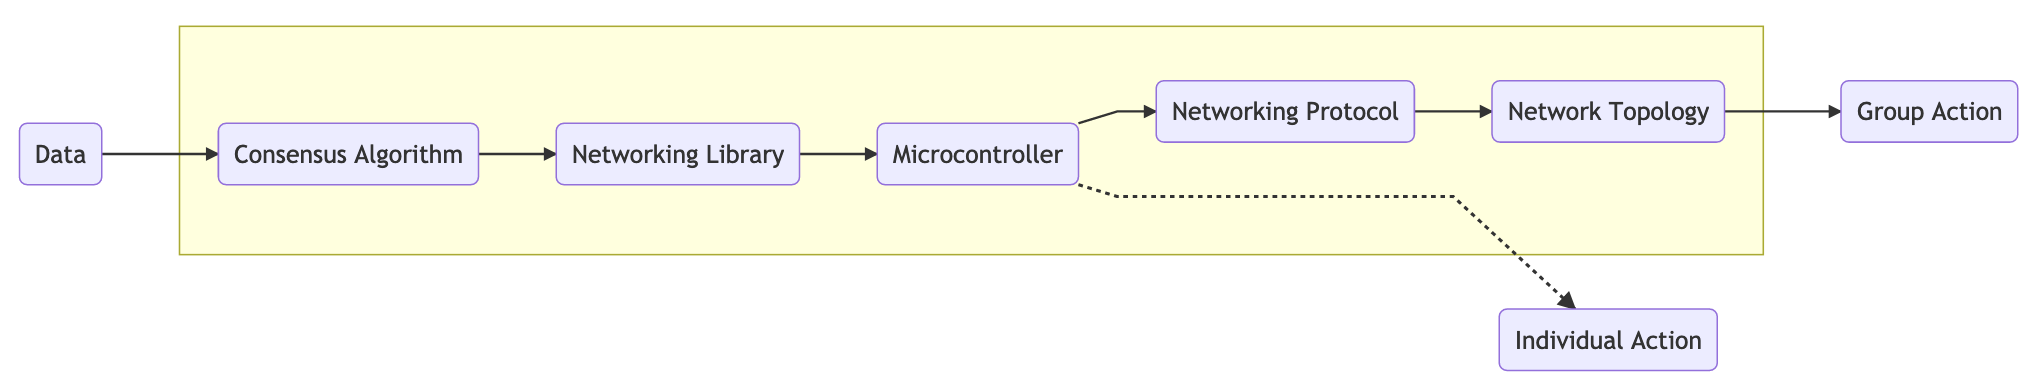
\includegraphics[width=0.95\columnwidth]{final-proposal/images/blackbox.png}
    \captionof{figure}{A black box diagram for each node of the system}
    \label{fig:black_box}
\endgroup

\subsubsection{Networking Protocols}
There are a plethora of network types for communication between industrial nodes, such as control area networks (CAN), Profibus, and Modbus \cite{lee2007comparative}. However, wired communications limit the flexibility of the nodes attached, especially in cases where these nodes are mobile. Hence, we turn to wireless networks, where there are four dominant protocols: Bluetooth, Ultra-wideband (UWB), Zigbee, LoRa, and Wifi \cite{lee2007comparative, ti_lethaby2017wireless}.

Mesh networks are not limited to any one of these standards. In fact, "IoT-related wireless technologies [...] are extremely heterogeneous in terms of protocols, performance, reliability, latency, cost effectiveness, and coverage",  \cite{iot_survey_cilfone2019wireless}. Each standard has its niche of operation: IoT devices may employ the IEEE 802.15.4 standard or Bluetooth for short-range communications, whereas mid to long-range communications may make use of IEEE 802.11, which was amended in 2011 to support mesh networks \cite{ti_lethaby2017wireless, iot_survey_cilfone2019wireless}. Figure \ref{fig:comparison_protocols} shows a comparative performance analysis of LoRa, Zigbee, Wifi, and Bluetooth, highlighting how each protocol has its strengths and weaknesses.

\begingroup
    \centering
    \medskip
    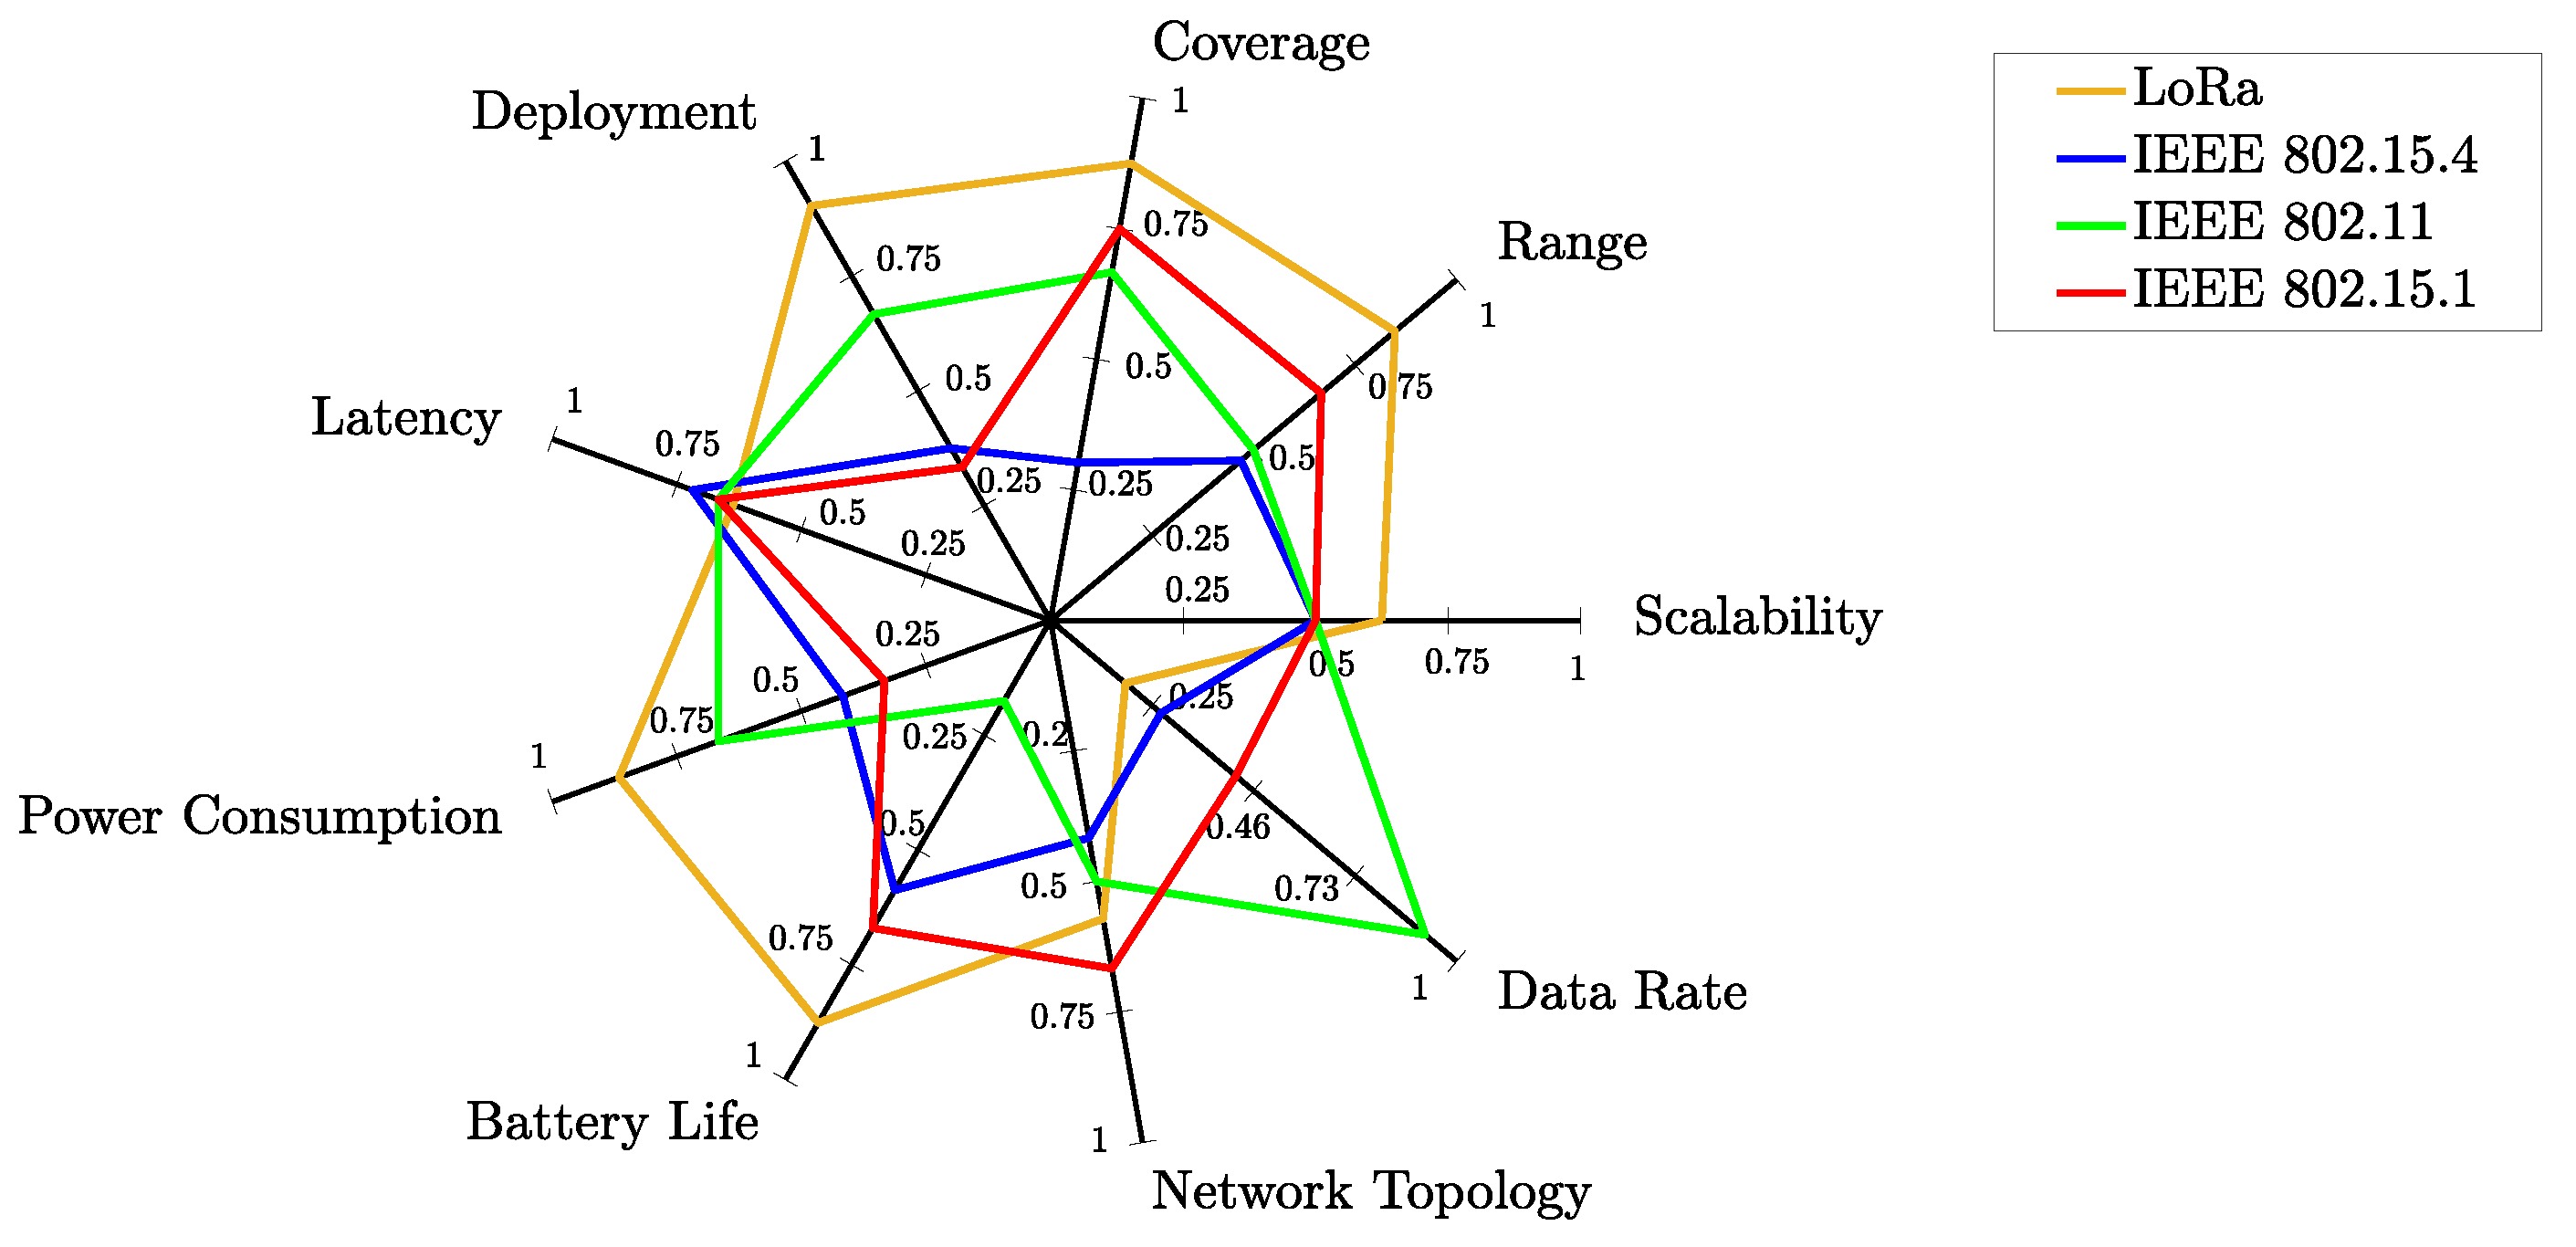
\includegraphics[width=0.85\columnwidth]{final-proposal/images/comp_perf_analysis.png}
    \captionof{figure}{Comparative performance analysis of four protocols. \\Source: Adapted from \cite{iot_survey_cilfone2019wireless}}
    \label{fig:comparison_protocols}
\endgroup

While the implementation of mesh networks and consensus algorithms are agnostic to the protocol underneath, it is important to address these concepts in the context of real-world constraints. Current IoT research "assumes that the devices are equipped with low-power IEEE 802.15.4 (Zigbee) transceivers" \cite{disney_glaropoulos2013enhanced}. Yet, a significant portion of deployed embedded systems and consumer electronics carry IEEE 802.11 compatible hardware \cite{disney_glaropoulos2013enhanced}. 
The "wide penetration of IEEE 802.11" \cite{disney_glaropoulos2013enhanced} then makes it the more attractive choice because hardware does not need to be redeployed to support newer standards. Despite 802.11's notoriety as a high power consumer, research indicates that additional firmware controlling the sleep scheduling can help lead to significant energy savings \cite{disney_glaropoulos2013enhanced, barghi2019practicalpower}

Furthermore, 802.11 has built-in support for mesh networks as a result of the 802.11s amendment. The amendment describes mesh stations (mesh STAs) and their ability to link with one another without the requirement of a central AP; rather, certain nodes may act as mesh access points (MAP) to connect to another network \cite{iov_wu2016internet, optical_zeitgeist_laboratory_2011}.

Given 802.11's ubiquity and built-in support for mesh networks, we found it fit to work with an 802.11-based network.

\subsubsection{Consensus Algorithms}
\label{conceptualization_consensus}
With the rapid increase in adoption and development of distributed \& multi-agent systems, achieving a consensus across these systems became an important issue because of the high potential for scalibility \cite{Ge_Han_Ding_Zhang_Ning_2018}. Achieving consensus across such systems allow autonomous air vehicles, cooperative IoT devices, sensor networks to be built at a scale. 

The distributed consensus algorithms can be classified into three categories based on their hierarchical structure: \emph{leaderless consensus algorithms}, \emph{leader-following consensus algorithms}, and \emph{containment control algorithms} \cite{consensus_systems_survey}. In \emph{leaderless consensus algorithms}, there are no leaders and the nodes within the system are expected to asynchronously converge on a target \cite{Ge_Han_2017}. However, in \emph{leader-following consensus algorithms}, there is a leader node that orchestrates the actions of the rest of the network. Finally, in \emph{containment control algorithms}, there might be more than one leader to orchestrate different types of operations within the system. A visualization of the different types of consensus algorithms can be seen in Figure \ref{fig:consensus_types_detailed}, where green circles are the leaders in the system and orange lines represent the logical connections between the consensus members.

\begingroup
    \centering
    \medskip
    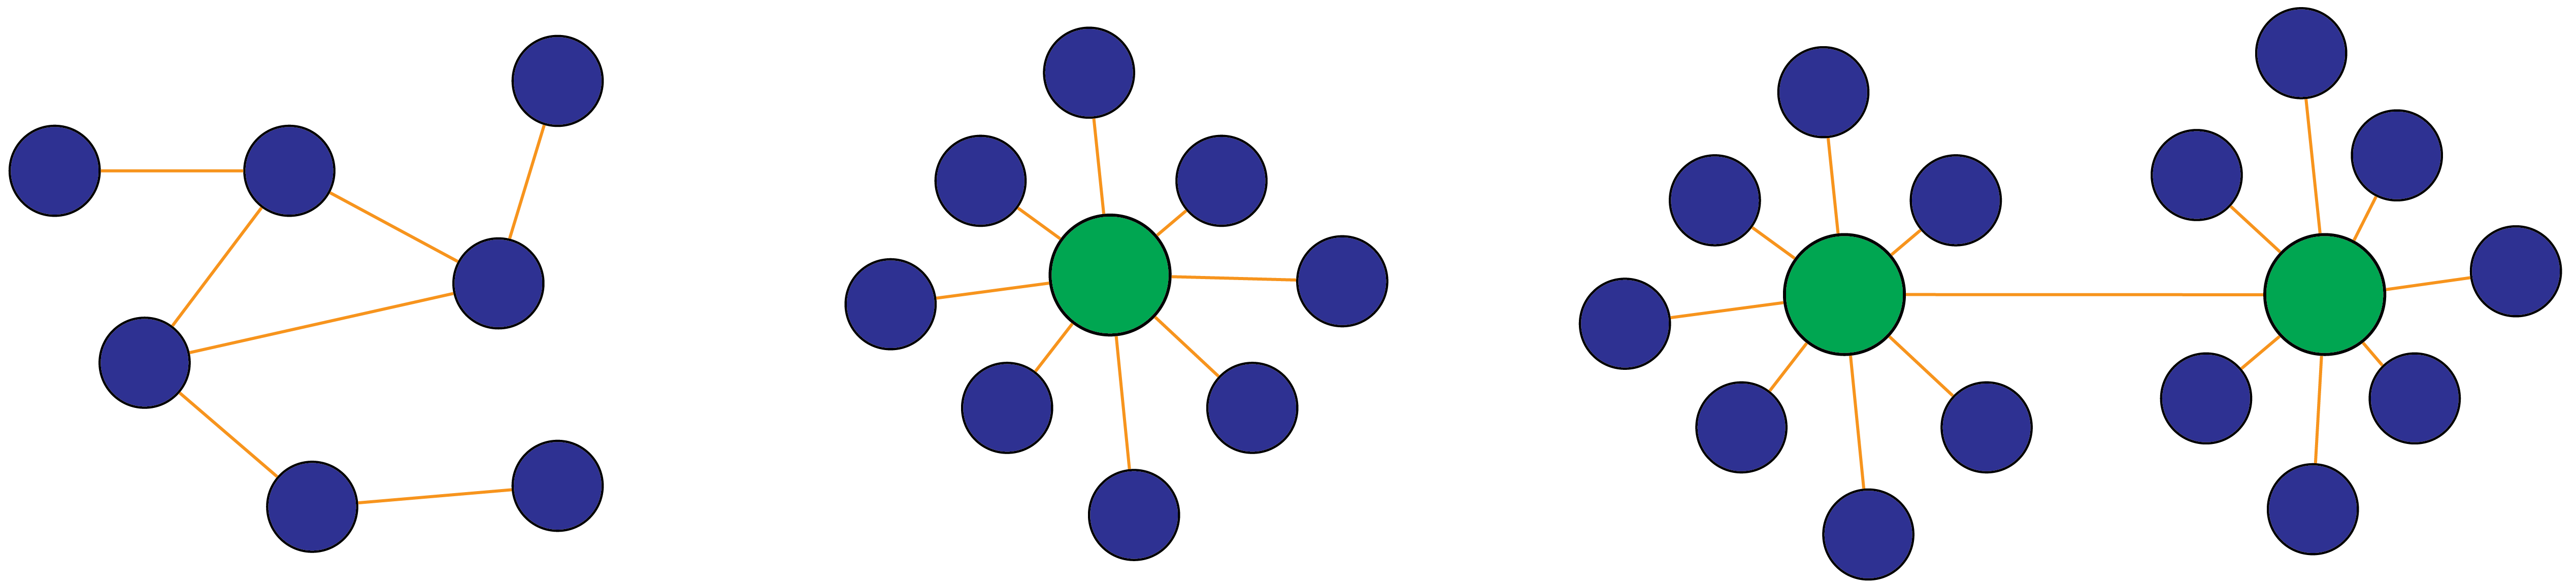
\includegraphics[width=0.75\columnwidth]{final-proposal/images/consensus_types.png}
    \captionof{figure}{Left: A leaderless consensus algorithm, Middle: A leader-following consensus algorithm, Right: A containment control algorithm}
    \label{fig:consensus_types_detailed}
\endgroup

The distributed consensus algorithms can also be classified into two categories based on when they transfer information to reach a consensus: \emph{time-triggered consensus algorithms} and \emph{event-triggered consensus algorithms} \cite{consensus_systems_survey}. In \emph{time-triggered consensus algorithms}, the nodes in the system initiate the information transfer once a set amount of time elapses. Additionally, if the consensus algorithm is asynchronous by design, each node can have a randomly set time duration before they send information. On the other hand, in \emph{event-triggered consensus algorithms}, the nodes in the system initiate information transfer when an external event occurs. A visualization of the different types of consensus algorithms can be seen in Figure \ref{fig:consensus_time_based_and_evevent_based}, where orange circles represent the timer of the nodes, green arrow represents the external event trigger, and red arrows represent the information transfer.

\begingroup
    \centering
    \medskip
    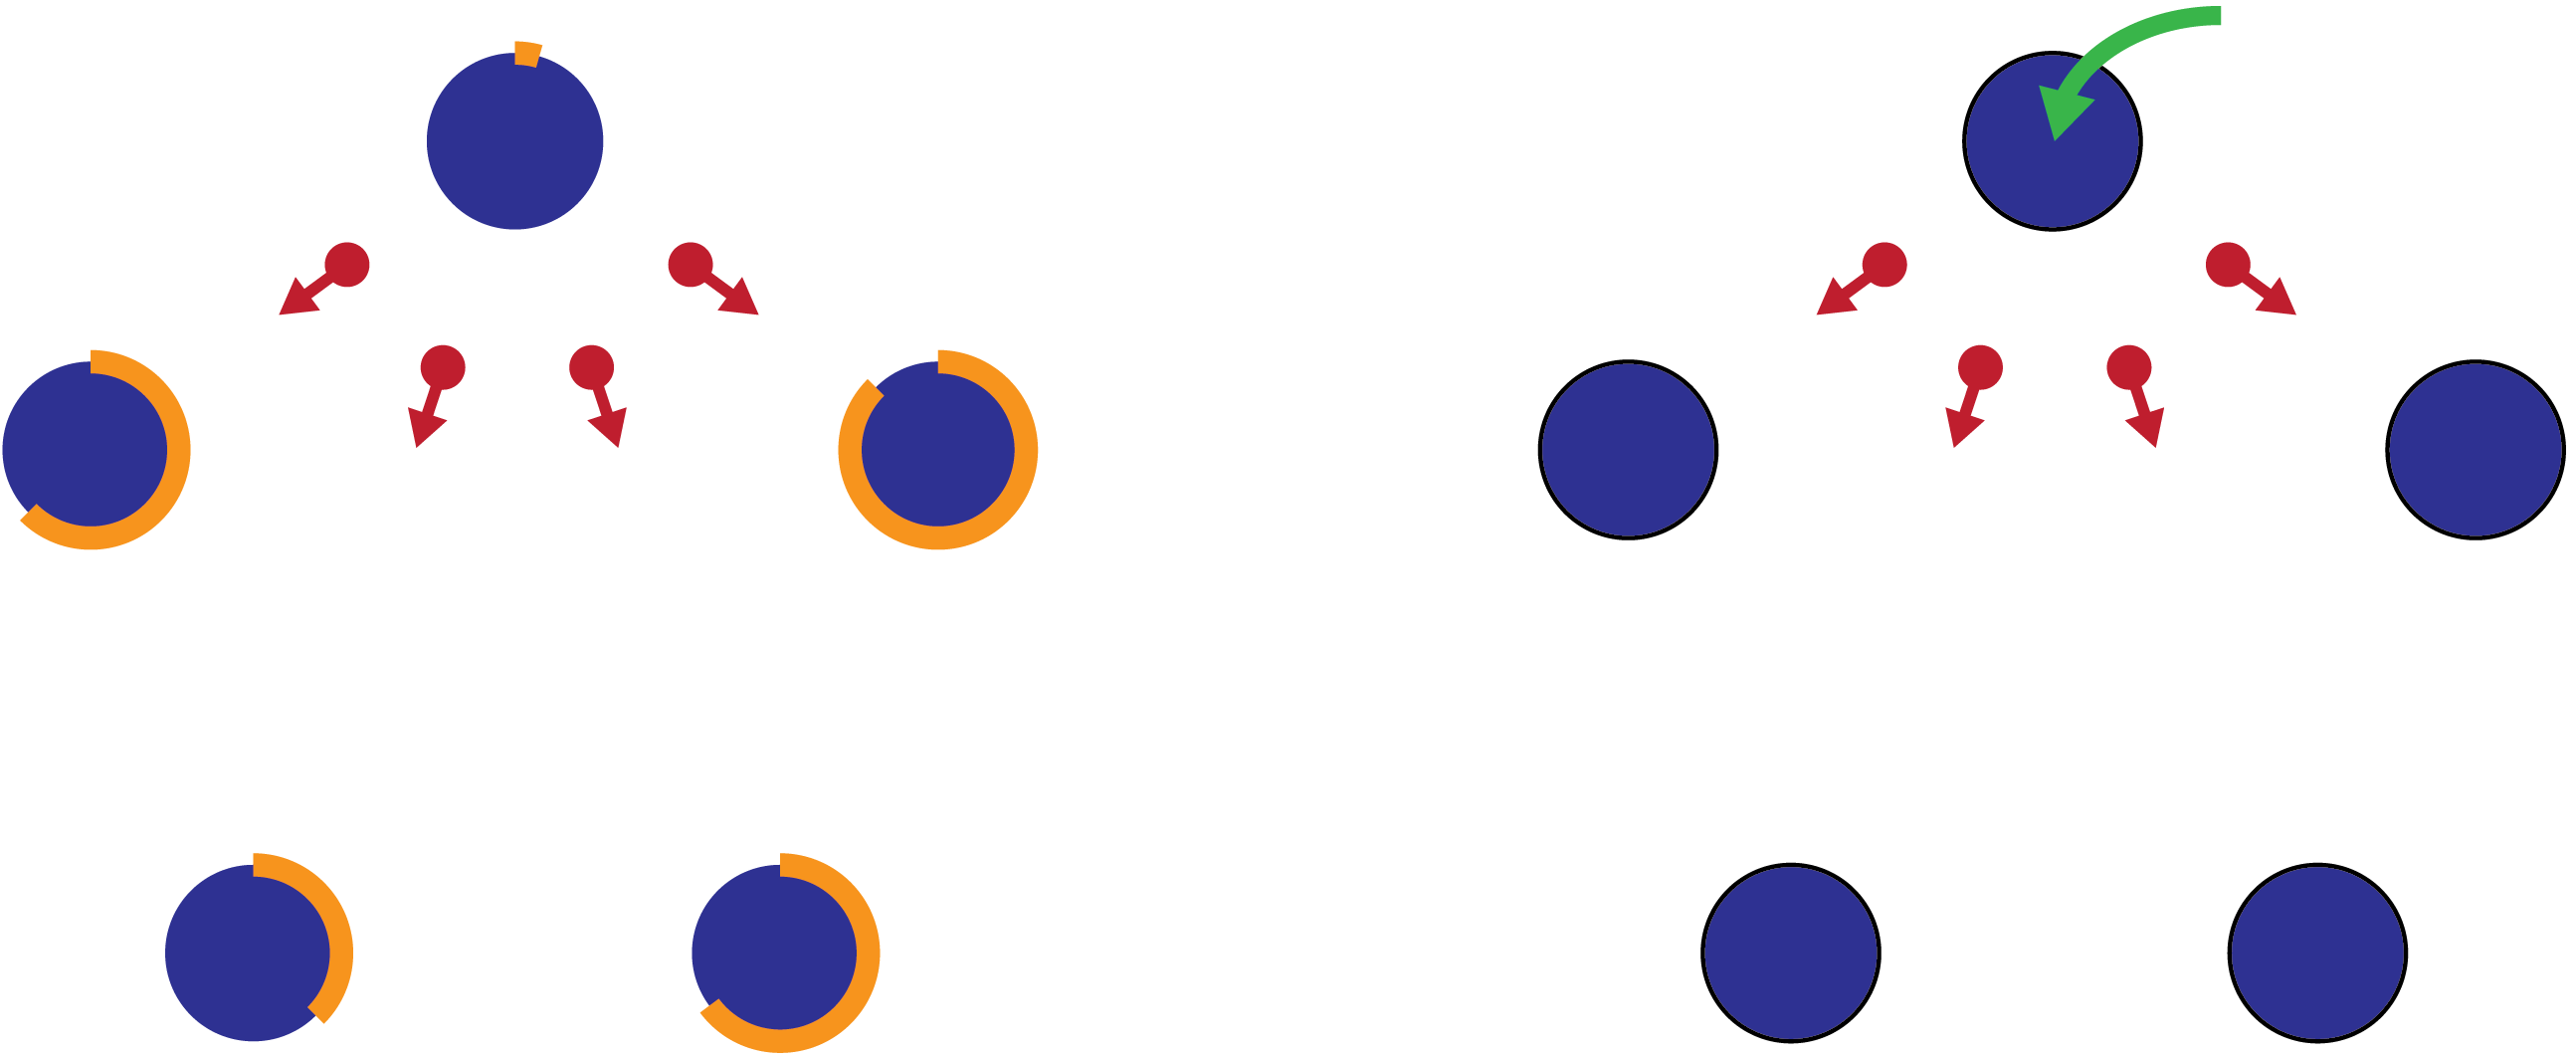
\includegraphics[width=0.45\columnwidth]{final-proposal/images/consensus_time_based_and_evevent_based.png}
    \captionof{figure}{Left: A time-triggered consensus algorithm exchanging messages when the timer goes off, Right: An event-triggered consensus algorithm exchanging messages when an event occurs (green arrow)}
    \label{fig:consensus_time_based_and_evevent_based}
\endgroup

Paxos and Raft are among the most popular \& practical distributed \emph{time-triggered} and \emph{leader-following} consensus algorithms available \cite{paxos_vs_raft}. Paxos has been the industry's first choice since it was published even though the way it works is not intuitive and difficult to understand. Since the Raft consensus algorithm aims to be simple and easy to understand \cite{raft_paper}, it is gaining more and more popularity in the industry. Furthermore, the Raft consensus algorithm aims to abstract the way the underlying technology works and not make it specific to a system \cite{paxos_vs_raft}. As a result, the Raft consensus algorithm is more suitable for experimenting and implementing on non-traditional topologies like mesh networks.

\subsubsection{Microprocessors}
Microcontroller units (MCUs) are a hefty consideration for any IoT solution. Unsurprisingly, there is a large variety of MCUs at different levels of "memory, power, computational capability, architecture etc." \cite{bansal2020iotsurveydevices} for various applications. These devices sit at different levels of the IoT ecosystem, implying that not all devices are required to be homogeneous in their capabilities. For discussion purposes, we adopt the classification system described in Bansal & Kumar's survey of IoT technologies \cite{bansal2020iotsurveydevices}. Class 0 devices may have 1-50KB of RAM with clock speeds below 100MHz, class 1 devices range from 100KB-100MB of RAM with clock speeds between 100MHz-1.5Ghz, and class 2 devices generally have resources greater than those of class 1 \cite{bansal2020iotsurveydevices}. Generally speaking class 0 devices such as the TELOSB are employed for Wireless Sensor Network (WSN) use-cases to collect data and perhaps perform simple actuation. On the other hand, class 1 devices, such as the well-known Raspberry Pis, are more suitable for coordination, media processing, data filtering tasks, etc.

Given our design constraints, namely dynamic topology and decision making capabilities, we would expect this system to work with embedded systems on mobile technologies such as drones, vehicles, and rovers. While such devices are often fitted with class 2 devices, the goal of our project is to be able to deploy such a networking ability on class 1 devices as well. Espressif's ESP8266 chip stands out as an option: the chip is designed to be a Wifi chip with a focus on low-cost and minimal peripherals. The MCU operates between 80-160MHz and has 50KB of SRAM with up to 16MB of external flash memory \cite{espressif:esp8266}, so it is on the lower-end of the class 1 category. Moreover, there is a decent open-source community dedicated to the MCU and Espressif has released a mesh networking software development kit (SDK) for its chips with detailed documentation \cite{esp-mesh-docs}. 


\subsection{Problem Statement}
%   Problem Statement
    % Clarify the scope of the problem [kinda done]
    % Project Aim [done]
%%%%%%% %%%%%%% %%%%%%% 

The of this Capstone Project is to design and develop a resilient wireless mesh network architecture coupled with a consensus algorithm for low-power embedded devices in dynamic topologies, demonstrated using 802.11-based ESP8266 boards.

We aim to create an open-source software library that anybody could incorporate in a system which requires nodes to work autonomoulsy together. We plan to demonstrate our software library through prototype boards that will each consist of an ESP8266 MCU, power sensors, and LEDs. Our software library will be installed on these boards to enable them to form a mesh network and run the Raft consensus algorithm. We will show how a signal propagates in the Raft consensus algorithm within the mesh network using LED lights as shown in Figure \ref{fig:mesh_signal_propagation}. We will also demonstrate how the network can realign \& recover itself by turning on and off randomly selected ESP8266 microchips.

\begingroup
    \centering
    \medskip
    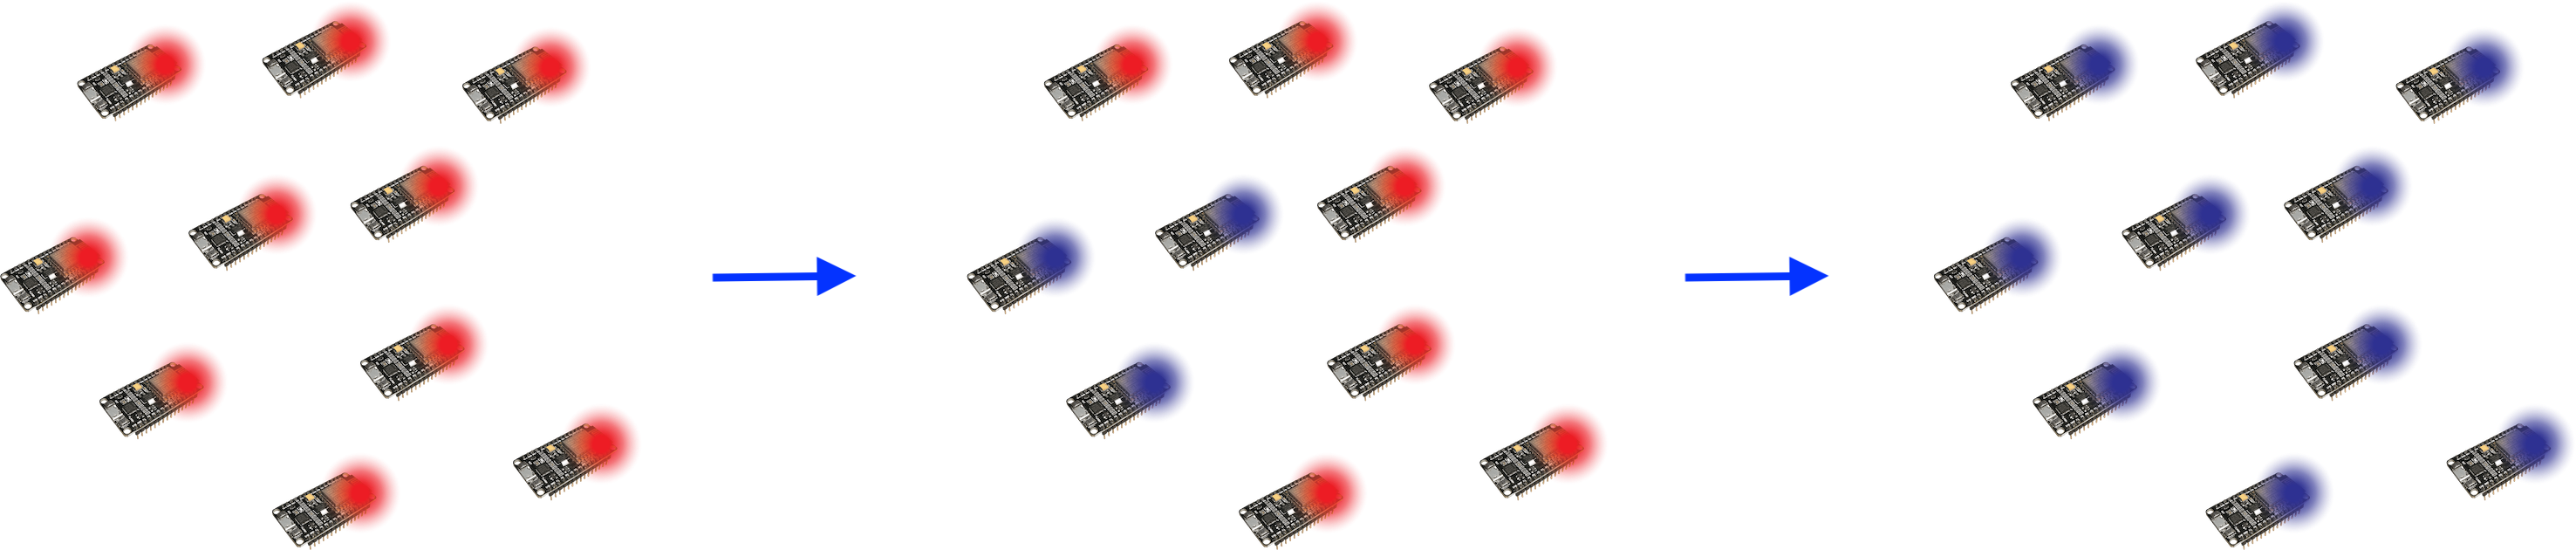
\includegraphics[width=\columnwidth]{final-proposal/images/mesh_signal_propagation.png}
    \captionof{figure}{An ESP8266 cluster transitioning to the blue state from the red state using our software library. Red and blue LEDs are used to represent the states.}
    \label{fig:mesh_signal_propagation}
\endgroup